%%
%% IP3R_Models.tex
%% Login : <hoang-trong@hoang-trong-laptop>
%% Started on  Wed Sep  2 15:42:41 2009 Hoang-Trong Minh Tuan
%% $Id$
%% 
%% Copyright (C) 2009 Hoang-Trong Minh Tuan
%%

\chapter{IP3R models}
\label{chap:ip3r-models}

\def\er{{\text{ER}}}
\def\cyto{{\text{cyto}}}

Many works on IP3R focuses on understanding the mechanism leading to calcium
oscillations (Sect.\ref{sec:calcium-oscillation}). Hypotheses
\begin{enumerate}
  \item biphasic response of IP3R/channel
  (Sect.\ref{sec:IP3R-biphasic-behavior}) to the cytosolic calcium is enough to
  induce calcium oscillations.
  
  \item 
\end{enumerate}

Based on Shuai et al. model~  \citep{shuai2007kmip3r}
(Sect.\ref{sec:shuai_2007}), the opening of a single channel requires the
opening of either 3 or 4 subunits. In turns, the opening of a subunit requires
the binding of an IP3, and biphasically modulated by  $\Ca$,, i.e. one $\Ca$
-binding will activate and two $\Ca$ -binding will inactivate. It means that
small elevation of [$\Ca$] promote subunit opening, while high elevation of
[$\Ca$] results in inactivation~\citep{bezprozvanny1991ip3r}.
In essence, the opening of a single IP3R subunit requires the binding of both
IP3 and an activating  $\Ca$, but not the inhibitory  $\Ca$. 
% For a complete
% reference on IP3R, read Chapter 22 on ThermoStatistics book.

There are quite a few number of kinetic models have been developed so
far\citep{atri1993spm}. However, there are significant differences in
behaviors to experimental data in their native environment of the
nuclear envelope, and only a few incorporated data obtained on nucleus
envelope. Recent works mainly use single-pool model, in which the release of
 $\Ca$ is modulated by both IP3 and  $\Ca$. 


% 
% \section{Introduction}
% \label{sec:IP3_intro}
% 
% 
% 
% 

% \section{Facts}
% \label{sec:facts}



\section{Calcium blips, puffs, waves}
\label{sec:blips}
\label{sec:puff}
\label{sec:calcium-release-IP3R}

The three levels of $\Ca$ releases via IP3R are given as follows.
\begin{enumerate}
  
  \item {\bf blips}:

The $\Ca$ release from the opening of a single channel is known as {\bf blips}
\citep{parker1996eei}

  
  \item {\bf buffs}

the $\Ca$ release from multiple channel opening is
known as {\bf buffs} which is a local transient restricted to clusters
containing several $\IPthreeR$ \citep{parker1996cta, parker1996eei}. 
  
  \item {\bf waves}


This InsP3-mediated Ca2+-release pathway involves positive and negative feedback
that often results in multiple cycles of release (oscillations), followed by
reuptake of Ca2+ into the ER as well as extrusion of Ca2+ across the PM.

Finally, when all release sites are activated, it causes a global $\Ca$
transient that leads to $\Ca$ wave propagating throughout the cell
\citep{bootman1997cwc, callamaras1998}.
Chap.\ref{chap:calcium_waves_IP3R} discusses
modeling of calcium waves.

\end{enumerate}


IP3 (Sect.\ref{sec:IP3}) $\leftarrow$ (Ca2+ PLC - Sect.\ref{sec:PLC})
Calcium has a biphasic effects on opening probability of IP3R
(Sect.\ref{sec:IP3R-open-probability}).
% 
% \begin{enumerate}
%   \item Purkinje cells of the cerebellum \citep{bezprozvanny1991} 
% 
% \end{enumerate}




\subsection{Conductance levels}
\label{sec:IP3R-conductance-level}

In previous models, the activation of ion channels are assumed to be all-or-none
manner, in which there is only two levels of ion conductance (on or off).

\textcolor{red}{IP3R was observed to have 4 conductance levels} in
Purkinjecells of {\it cerebellum}, with opening to level three
predominating and level 0 is no conductance (close
channel)~\cite{watras1991ip3r}. Measuring the currents at different
holding potential at which the channel active, there were 4 different
levels of currents observed for each holding potential.  

One explanation for the 4 conductance levels is the incorporation of 4
independent subunits in the tetrameric channel complex. Calcium
release and single-channel data suggest there are functional
interaction among the subunits~\cite{watras1991ip3r}.  The conductance
times was 60ps (picro-second), as shown in
Fig.~\ref{fig:IP3R_4conductance}(B), with 20ps for each level. 
\begin{itemize}
  \item 60pS means 1.8pA at 0mV. 
\end{itemize}

The current steps from level 1 to 2 to 3 followed by an abrupt return to zero
current, as shown in Fig.~\ref{fig:IP3R_4conductance} (A). As it is
difficult to distinguish level 1 from baseline noise;
\textcolor{red}{in many cases, level 1 was ignored and considered as
non-conductance state}.

In essence, probably, IP3R have 3 conductance levels. However,
computational models majorly use two conductance
levels~\cite{deyoung1992spip3}.

\begin{figure}[hbt]
 \centerline{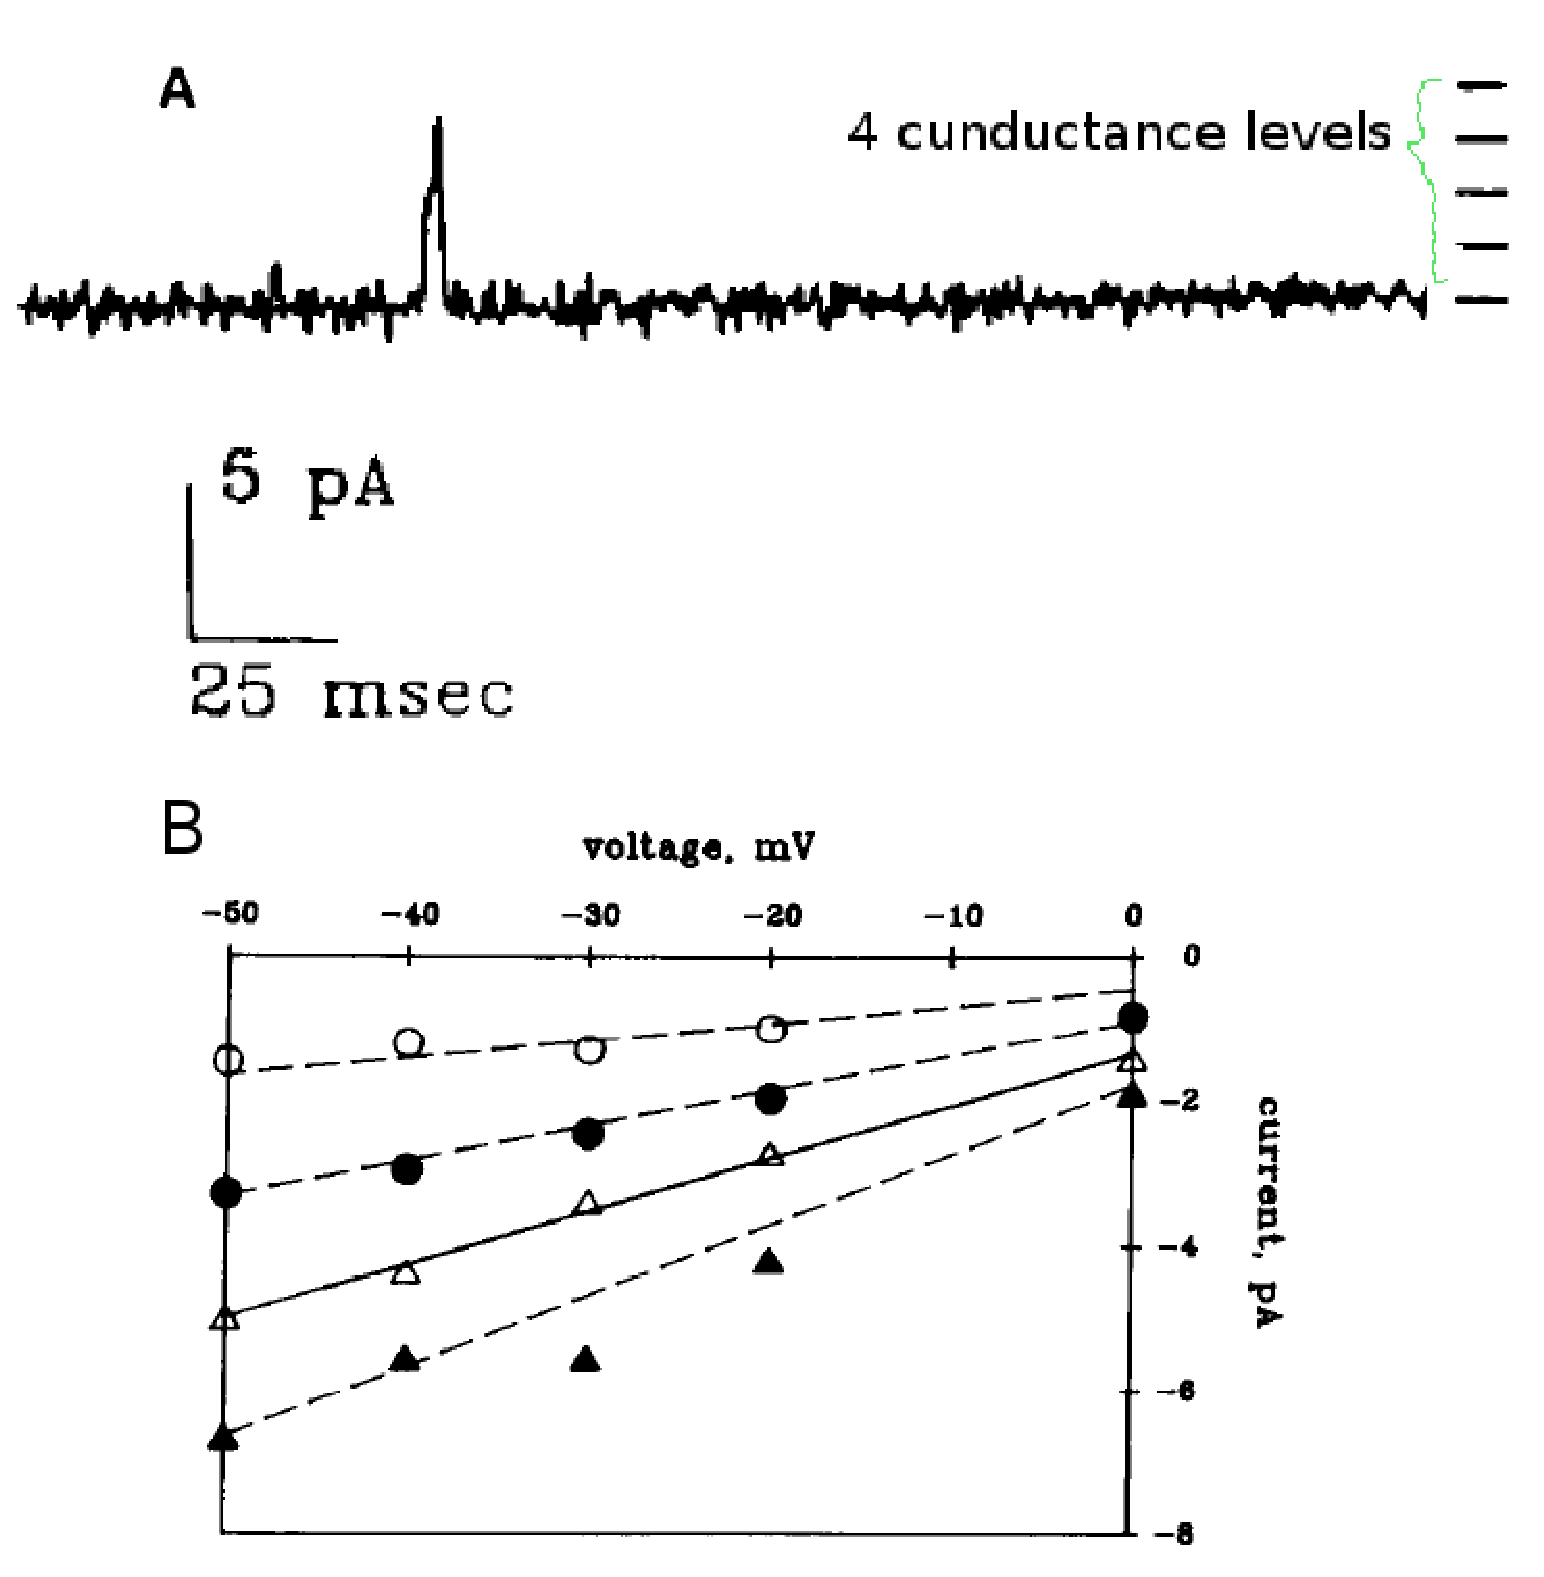
\includegraphics[height=5cm]{./images/IP3R_4cond.eps}, 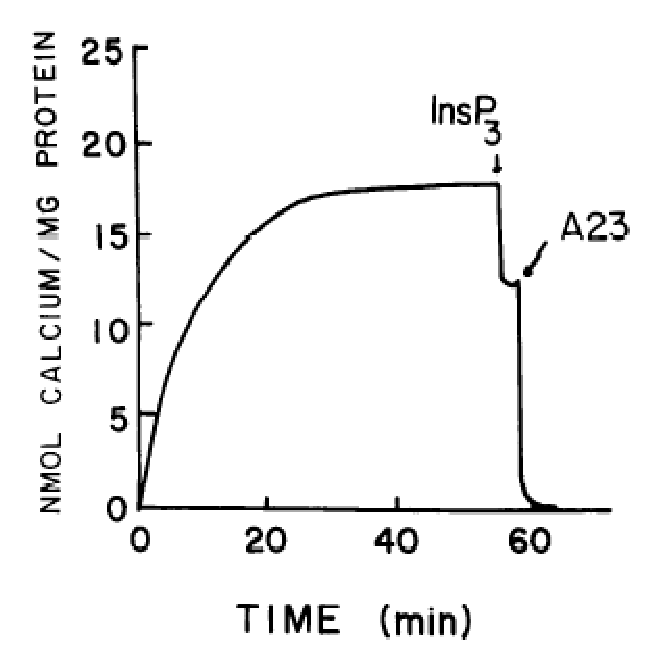
\includegraphics[height=5cm]{./images/IP3R_cond_time.eps}}
\centerline{         (A)   \hspace{20mm}   (B)    }
\caption{(A) 4 conductance levels in IP3R found in Purkinje cells of
  cerebellum; (B) conductance time for an IP3R}
\label{fig:IP3R_4conductance}
\end{figure}

% \begin{figure}[hbt]
%  \centerline{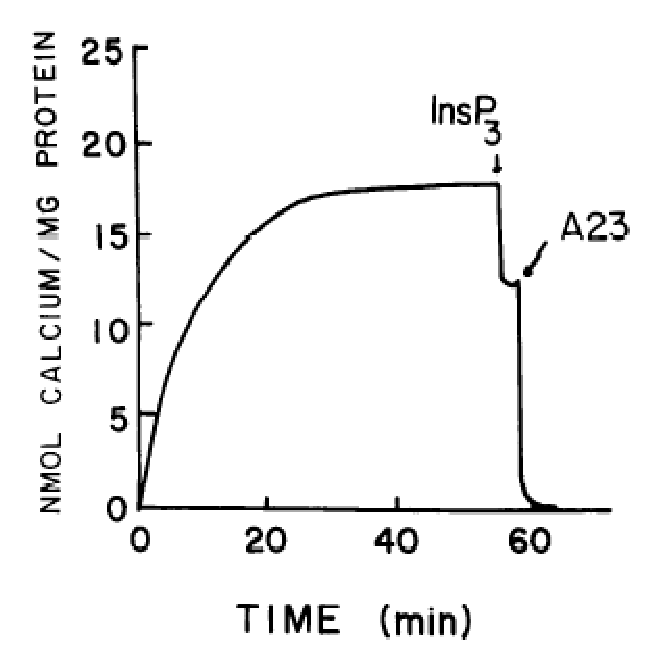
\includegraphics[height=5cm]{./images/IP3R_cond_time.eps}}
% \caption{Conductance time for an IP3R}
% \label{fig:IP3R_conduc_time}
% \end{figure}



\subsection{Open probability}
\label{sec:IP3R-open-probability}
\label{sec:IP3R-biphasic-behavior}

The opening of IP3R is more often than RyR due to the more sensitive to $\Ca$
level. First the opening of IP3R requires IP3 binding as the pre-condition.
IP3R open at the holding potential $-50mV$ with $2\mu M$
IP3~\cite{watras1991ip3r}. 

The opening probability then also change as a function of calcium
concentration; and calcium binding is required for the channel to open (in
Purkinje cell).
\begin{itemize}
  \item maximum Po is 15\%: \citep{bezprozvanny1991ip3r}
\end{itemize}

The opening probability $P_o$ of type 1 and 3 follows a biphasic dependency on
cytoplasmic free $[\Ca]$, suggesting the channels have two distinct types of
functional $\Ca$-binding sites: activating and inhibitory
\citep{mak1998,mak2001}.
\begin{itemize}
  \item Joseph et al. (1989): in cerebellum microsomal fractions with $\Kd$ of
  IP3-binding to microsomes membrane as a function of pH and extravesicular
  calcium concentration. (Sect.\ref{sec:Joseph-Rice-Williamson-1989})

  \item Parker - Ivorra (1990): a similar behavior found in IP3-sensitive store
  in Xenopus oocytes

  \item Finch et al. (1991) showed IP3-induced calcium efflux of $\Ca$ ions from
  microsomal vesicles was first enhanced, then inhibited as extravesicular
  calcium level increases from 100 nM to 100 $\muM$
  
  \item Bezprozvanny et al. (1991): in Purkinje cells with the peak of Po vs.
  $[\Ca]$ is at calcium level 0.25$\muM$.

The opening probability increase with calcium level, as long as $[\Ca] <
0.25\muM$; then it decreaes if calcium continues to increase.
  
\end{itemize}


Most of the developed IP3R models can explain the Ca2+ dependence of the open
probability (Po) of IP3R. Only a few model can accurately reproduce the IP3 dependence
of Po. 
\begin{itemize}
  \item  Mak et al. (2003) - Sect.\ref{sec:Mak_2003_IP3R}) with 14 parameters
  
  \item Ullah et al. (2012) - Sect.\ref{sec:Ullah-Mak-Pearson-2012-IP3R} with 
  
\end{itemize}


\begin{itemize}
  \item At $[\Ca]_i < 0.25\muM$, increase $\Ca$ leads to increase Po of
IP3R; and after reaching the peak, then decrease at $[\Ca]_i > 0.25\muM$.

  \item 
\end{itemize}


Data:
\begin{itemize}
  \item \citep{bezprozvanny1991ip3r} -
  Sect.\ref{sec:IP3R-opening-prob-Bezprozvanny1991}
\end{itemize}

\subsection{-- Hill equation}
\label{sec:IP3R-open-probability-Hill-equation}

The empirical biphasic Hill equation for steady-state opening probability of
IP3R is 
\begin{equation}
P_o = P_\max \left( 1+ \left(\frac{K_\act}{[\Ca]_i}\right)^{H_\act} \right)^{-1}
\left( 1 + \left( \frac{[\Ca]_i}{K_\inh}\right)^{H_\inh} \right)^{-1}
\end{equation}
with $P_\max$ is maximum channel open probability (under optimal $[\Ca]_i$ and
saturating [\IPthree]), $K_\act$ is the half-maximal activating $[\Ca]_i$,
$H_\act$ is activation Hill coefficient, $K_\inh$ is half-maximal inhibitory
$[\Ca]_i$, and $H_\inh$ is inhibition Hill coefficient.

\subsection{-- Pmax}

\begin{enumerate}
  \item In nuclear patch-clamp experiment, $P_\max = 0.8$. 
  
  $K_\inh \sim 40-50\muM$ in the presence of saturating [\IPthree]. However,
  this value should increase when [\IPthree] increase, i.e. more $\Ca$ is
  required to cause the inhibition. This can be formulated using an empirical
  Hill equation (in the presence of free [ATP] = 0.5 mM)
  \begin{equation}
  K_\inh = K^\infty_\inh \left( 1 + \left( \frac{K_\mIPthree}{[\mIPthree]}
  \right)^{H_\mIPthree} \right)^{-1}
  \end{equation}
  with half-maximal activating [\IPthree]: $K_\mIPthree \sim 50$ nM,
  $H_\mIPthree \sim 3$. $H_\inh \sim 3-4$ (indicating $\Ca$ inhibition is highly
  cooperative). 

  \item  
In Purkinjecells of cerebellum, maximum open probability observed
was $P_{max} < 15\%$ (using optimal concentration of
IP3)~\cite{watras1991ip3r}. 

At a fixed [IP3], the gating of an IP3R is modeled as the activity of an enzyme
with substrate is $\Ca$ and inhibitor is also
 $\Ca$.  With a fixed [IP3] at $0.2\mu M$, the
open probability for IP3R as a function of [$\Ca$] is a bell-shaped curve with
optimum open probability at [$\Ca$]=$0.25\mu M$~\cite{bezprozvanny1991ip3r}.

\end{enumerate} 

\subsection{Mean open time}
\label{sec:mean-open-time-IP3R}
\label{sec:IP3R-mean-open-time}


In Purkinkie cells of cerebellum, transition from open to closed state was
rapid, with mean open time less than 10ms~\cite{watras1991ip3r}. During this
time, mean open time to level three was $2.7msec$, longer than that for levels
one and two ($1.0ms$ and $1.6ms$), suggesting the channel is more stable at
level 3~\cite{watras1991ip3r}. This suggests that at level 3, three or four
subunits in a single channel are opened. 

Preliminary results suggested that the mean open time is quite constant at
different concentration of  $\Ca$. So, the increase in $P_o$ probably links to
the number of open channels per unit of times changes, to match with the
bell-shaped curve $P_o([\ce{Ca^2+}])$.





\subsection{Calmodulin-binding sites: $\Ca$ inhibition of $\Ca$ release}
\label{sec:ceca2+-inhib-ceca2+}
\label{sec:IP3R-inhibition}

Willems et al. (1990) suggested that [\ce{Ca^2+}] in the range
$0.1-0.2\mu M$ do not inhibit the release, and that [\ce{Ca^2+}] must
reach the levels $2-3\mu M$ before inhibition occurs.

Parker and Ivorra's work showed that at least 3 time scales operating
in Xenopus oocytes: 
\begin{itemize}
\item a rapid (0.2-0.5s) release of $\Ca$ from IP3-sensitive pool

\item a slower inhibition (2-3s) of $\Ca$ release by \ce{Ca^2+}
  inhibition

\item a longer recovery process (14-20s)
\end{itemize}

Calmodulin (CaM - Sect.\ref{sec:calmodulin}) was one of the first protein
identified to interact with IP3R in a calcium-dependent manner (Yamada et al.,
1995). IP3R has 2 binding sites for CaM at N-terminus site
\begin{enumerate}
  \item one of which is $\Ca$-dependent, and is found on IP3R type 1 at residue
  1564-1589.
  
NOTE: There is CaM-binding site on IP3R type 3.
  
  \item one in the extreme N-terminus which is $\Ca$-independent (Patel et al.,
  1997) and is found at residue 6-159.
  
The N-terminus was further mapped to adjacent regions: residue 49-81 and 106-128
(Sienaert et al., 1997).


\end{enumerate}


Calmodulin binding to Calcium appears to be required for $\Ca$-dependent
inhibition (Michikawa et al., 1999; Hirota et al., 1999). However, in other
single channel studies that used point mutation to eliminate the binding of CaM
at $\Ca$-dependent binding site, it does not remove the $\Ca$-dependent
inhibition effect (Zhang and Joseph, 2001; Nosyreva et al., 2002).

The result suggested that only one site is responsible for $\Ca$-dependent
inhibition and this is $\Ca$-independent CaM-binding site (Patterson et al.,
2004). However, calmodulin may also play some physiological roles in that it
influences the binding of IP3 to IP3R. 

In the studies with agents to compete CaM from IP3R, they showed that CaM
binding to IP3R can be taken away by calmodulin-binding peptides (Kasri et al.,
2006), e.g. myosin light chain kinase peptide which has high-affinity to CaM.


\subsection{Calderin (CaBP)}

Calderin (CaBP) also interact with IP3R at CaM-binding site



\section{Single Channel Current}


\citep{mak1994, mak1998}

\section{IP3R models}
\label{sec:IP3R_models}

Some earliest works assumed a two-pool model, i.e.
there are two distinct $\Ca$ stores: one with IP3-sensitive and the other with
$\Ca$ sensitive~\cite{dupont1989ip3}. In this approach, the IP3 production leads
to the release of $\Ca$ from an IP3-sensitive store and the released $\Ca$
induce the release of $\Ca$ from a different \ce{Ca^2+}-sensitive store,
possibly via RyRs. The crucial assumption with these models is that the
concentration of $\Ca$ inside the IP3-sensitive store remains constant, as the
store is quickly refilled by $\Ca$ from extracellular medium. On 2004,
\citep{sneyd2004} performed a comparision between three models:

Why studying blip events (Sect.\ref{sec:blips}) is difficult?
\begin{enumerate}

  \item Most of the experimental data of \tIPthreeR were obtained from
  patch-clamp and bilayer recording of single \tIPthreeR channels under
  conditions where charge carrier is not $\Ca$ ions and $\Ca$ on the cytosolic
  face is clamped to a fixed concentration by buffers. So, the effect of $\Ca$
  feedback has not been observed correctly.

  \item Opening of one \tIPthreeR usually triggers the opening of multiple
adjacent channels in the cluster.

  \item endogenous buffers also affect the magnitude, kinetics and spatial
distribution of cytosolic $\Ca$ signals
\end{enumerate}
\citep{shuai2008} (Sect.\ref{sec:shuai_2008_Ca-feedback}) carried out that study
{\it in silico}.

 The biphasic positive and negative feedback of $\Ca$ ions on \tIPthreeR gating
 underlies a complicated $\Ca$ signaling on channel gating.





\section{Eigen et al. (1968) - generic allosteric model}
\label{sec:eigen1968-IP3R}

Eigen's "general allosteric model" has 55 states for a tetrameric channel in
which each subunit can bind a single ligand and has two major conformations
(Eigen, 1968).

However, the model is too complicated for most type of simulations.

\section{Joseph - Rice - Williamson (1989)}
\label{sec:Joseph-Rice-Williamson-1989}
\label{sec:IP3R-Joseph-Rice-Williamson-1989}

Rat cerebellum membrane contains a significant amount of IP3R
(Sect.\ref{sec:IP3R-distribution}). The binding of IP3 to IP3R on rat cerebellum
membrane has been shown to be a function of pH level and $\Ca$ concentration
(Worley et al., 1987); where calcium functions as an inhibitor to the binding of
IP3 to the receptors on the membrane.
Calcium inhibit by binding to the receptors.

Here, the authors studied the binding of IP3 to cerebellum microsomes as a
function of pH level and extravesicular $\Ca$ concentration
\citep{joseph1989ip3}.
They both shows that
\begin{itemize}
  \item high pH facilitate the binding (i.e. low Kd): affect the apparent
  binding affinity (i.e. increase $\Kd$), but not the maximal binding capacitiy
  (i.e. keep the same B$_\max$).

\begin{verbatim}
                             Kd (nM)                Bmax (pmol/mg)
pH=8.3; no Calcium        64.2 +/- 7.7              25.2 +/- 1.7
pH=8.3; 1uM Calcium       220      8.3              27.4     1.8
pH=7.2; no Calcium        145.2    22.8             31.3     4.4
pH=7.2; 1uM Calcium       542                       36.9
\end{verbatim}

  \item low concentration of $\Ca$ inhibit the binding

At low concentration of IP3, i.e. 15 nM, the amount of bound IP3 is reduced with
the increase of free calcium from 0.1$\muM$ to 1.0$\muM$ (complete within
5 seconds). The inhibition of low $[\Ca]$ was most marked when IP3 level is
below a sub-optimal concentration.

At higher IP3 concentration, i.e. 150 nM, more calcium (which is about
30$\muM$) is required to obtain 50\% inhibition.

In brain microsomes and neuronal cell lines, the effective range of $[\Ca]$ is
between 1 and 50 $\muM$.

  \item 
\end{itemize}



\section{Bezprozvanny et al. (1991): fixed IP3, single-channel}
\label{sec:IP3R-opening-prob-Bezprozvanny1991}

Using data from planar lipid bilayer, single-channel IP3R activity was monitored
using 2 $\muM$ IP3, 330 $\muM$ AMP-PCP, and 0 mV potential. $\Ca$ level is
changed from 0.1$\muM$ to 5.0 $\muM$. Based on the condition of fixed IP3 level,
with max-opening probability observed was 15\% and mean open time 3ms, they
build the model IP3R .

Despite the 4 conductance levels (20pS to 60pS with 20pS increment at each
level) and that 60pS maps to 1.8pA at 0mV
(Sect.\ref{sec:IP3R-conductance-level}), the authors chose 1pA as the threshold
for channel opening (which includes opening from level 2 to 4)
\citep{bezprozvanny1991ip3r} and fitted the opening probability at steady-state
by the functional form using Hill-based equation
(Sect.\ref{sec:IP3R-open-probability-Hill-equation}).



\subsection{2-site single subunit model}

The {\bf two-site model} for non-competitive cooperative binding
(Sect.\ref{sec:non-competitive-two}) was utilized:
one for $\Ca$ activation and one for $\Ca$ inhibition; and the steady-state
opening probability $P_o$ is
\begin{equation}
  \label{eq:329}
  \begin{split}
      P_o &= P_{max} \frac{[\ce{Ca^2+}]}{K_M + [\ce{Ca^2+}]}
      \frac{1}{1+\frac{[\ce{Ca^2+}]}{K_i}} \\
      &= P_{max} \frac{[\ce{Ca^2+}]K_i}{([\ce{Ca^2+}]+K_M)([\ce{Ca^2+}]+K_i)}
  \end{split}
\end{equation}
Given $K_M$ and $K_i$ as
the association (binding) constants for substrate and inhibitor, respectively.
 $P_{max}$ is the maximum open probability observed. However, the
dash curve drawn from this equation does not fit to the experimental
data very well, as shown in Fig. \ref{fig:bezprozvanny1991}.

% This is an uncompetitive cooperative binding mechanism. Bezprozvanny et al.
% \cite{bezprozvanny1991ip3r} modelled an IP3R with two different binding sites,

\begin{figure}[hbt]
  \centerline{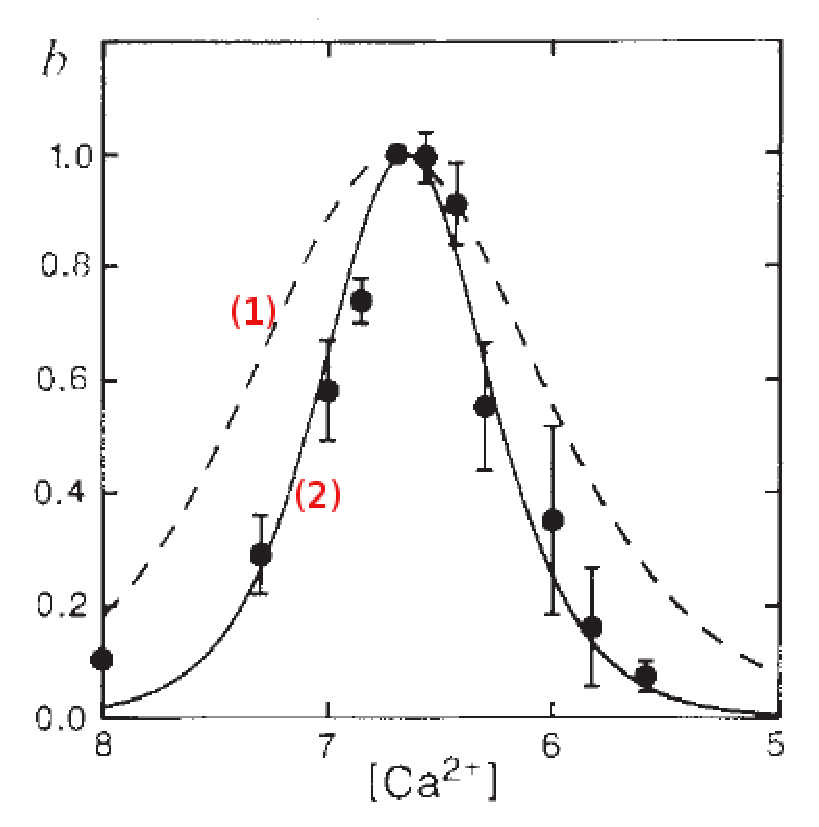
\includegraphics[height=5cm]{./images/bezprozvanny1991_bellshape.eps}}
  \caption{
  The data shows the opening probability as a function of -log[Ca]. Here, 
  (1) dashed-line curve was generated from
    eq.~\eqref{eq:329}, (2) curve was generated from
    eq.~\eqref{eq:330} and eq.~\eqref{eq:331}}
\label{fig:bezprozvanny1991}
\end{figure}

\subsection{2n-site single subunit model}

Then, Bezprozvanny et al. \citep{bezprozvanny1991ip3r} suggested that there
could be more than two binding sites, i.e. they assumed $n$ sites for
activation and $n$ sites for inhibition. $n$ is called Hill
coefficient (or $n_H$).
\begin{equation}
  \label{eq:330}
  P'_o =  P_{max} \frac{[\ce{Ca^2+}]^nK^n_i}{([\ce{Ca^2+}]^n+K^n_M)([\ce{Ca^2+}]^n+K_i^n)}
 \end{equation}
Fitting to the experimental data, the best fit was obtained with
$n=1.8, K_M=K_i=0.2\mu M$. It thus suggested that calcium binds
cooperatively to at least 2 sites to activate and to 2 other sites to
close the channel. 

\subsection{m-subunits (each with 2-site) model}

Another modification suggested by Bezprozvanny et al. was that an IP3R
is a complex with $m$ subunits operate independently. Each subunit
with one $\Ca$ activating binding site and one \ce{Ca^2+}
inhibitory binding site. Then, using the opening probability for one
subunit in eq.~\eqref{eq:329}, the opening probability for the channel
complex is the multiplication of the opening probabilities of those
$m$ subunits,
\begin{equation}
  \label{eq:331}
  P = (P_o)^m
\end{equation}

Fitting to the experimental data, the best fit for 2-site binding for each
subunit, the result was obtained with $m=2.7, K_M=K_i=0.2\mu M$. It thus
suggested that there are 3 subunits in an IP3R channel, each with 2-binding
sites.
This is the motivation for De Young-Keizer model which assumed 3 subunits in
every IP3R channel~\cite{deyoung1992spip3} (Sect.\ref{sec:de-young-keizer}).

% Even though, it is observed that there are 4 levels of conductance in
% which 3 levels corresponding to open channel, level 1 were ignored
% (considered as closed) as it's too close to baseline noise.

\section{** De Young-Keizer (1992) - single channel}
\label{sec:de-young-keizer}
\label{sec:IP3R-DeYoung-Keizer-1992}

De Young-Keizer model is one of the early and widely used {\it binding models}
on microscopic kinetics of IP3 and $[\Ca]_i$ on the gating of IP3R
\citep{deyoung1992spip3}. By ``binding'', we mean that the activation of IP3R
requires the binding of some agonists. 

This model was derived from two crucial features of IP3R that was discovered in
the early 90s and based on analysis from \citep{bezprozvanny1991ip3r}
(Sect.\ref{sec:IP3R-opening-prob-Bezprozvanny1991}) and from
\citep{joseph1989ip3} (Sect.\ref{sec:Joseph-Rice-Williamson-1989}); when the ER
membrane potential is zero.

\begin{itemize}
  \item At steady state, the open probability of the IP3R is a
  bell-shaped function of [\ce{Ca^2+}], with maximum open probability
  when [\ce{Ca^2+}] in the range 300-500 nM~\citep{bezprozvanny1991ip3r}.

% It became clear that for a step increase in [\ce{Ca^2+}], IP3R
% responses in an adaptive manner, first activating and subsequently
% inactivating. In other words, there is a biphasic regulation of
% [\ce{Ca^2+}] on IP3R.

\begin{figure}[hbt]
 \centerline{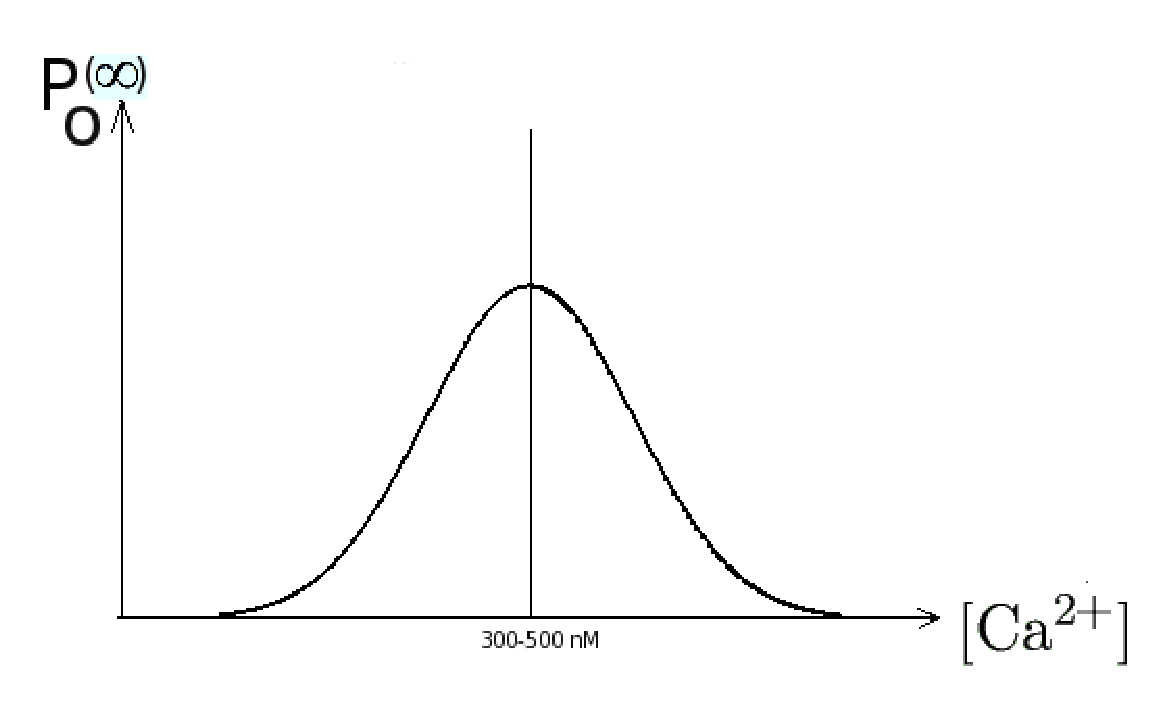
\includegraphics[height=5cm]{./images/Popen_IP3R.eps}}
\caption{Open probability of IP3R vs. calcium concentration at steady state}
\label{fig:Popen_IP3R}
\end{figure}

\item The opening probability of IP3R is also a function of [IP3]
\end{itemize}

It became clear that for a step increase in [\ce{Ca^2+}], IP3R responses in an
adaptive manner, first activating and subsequently inactivating. Adaptation of
the IP3R is now believed to result, at least in part, from the fact that $\Ca$
release not only induce its own release, but also inhibit it on a slower time
scale. This suggests there are at least two calcium-binding sites on IP3R: one
activating with higher-affinity and one inactivating with lower affinity.

\subsection{Assumptions}

\begin{enumerate}
  \item idealized closed-cell : exchange of Ca2+ between cytosol and
  extracellular is ignored. This is the scenario of Ca2+ free extracellular
  media; or Ca2+ pumps are inhibited.
  
They only model the diffusion of Ca2+ across ER membrane.

  \item The IP3R has 3 subunits -
  Sect.\ref{sec:ideas}
  
  \item 3 binding sites for each subunit: IP3 binding, Ca2+-activation binding, 
  and Ca2+-inactivation binding.

\textcolor{blue}{NOTE: There is no need for independent binding assumption of
the 3 binding sites}. So, IP3 binding rate is depending upon whether the
Ca2+-inactivation binding site is occupied or not; and Ca2+-inactivation binding
is depending upon whether the IP3 is bound or not.

   \item To reduce the complexity:
   
   The two binding processes (IP3 binding, and Ca2+-inactivation binding) are
   assumed independent from Ca2+-activation binding and vice versa. This gives
   rise to some symmetries to the binding rate matrix.
 
\end{enumerate}


\subsection{Ideas: m=3; 3-site}
%\subsection{Assumptions}
\label{sec:ideas}

Using the analysis from Bezprozvanny et al. (1991 -
Sect.\ref{sec:IP3R-opening-prob-Bezprozvanny1991}), a model using the kinetics
of 3 independent subunits for IP3R is assumed.

\textcolor{red}{ASSUME}: Each subunit has 3 binding sites: 1 for IP3, one
for Ca2+ activation, and 1 for Ca2+ inactivation; denoted as (X,Y,Z) in that
order.
% Each subunit has 3 binding sites: one IP3 binding site, one
%   high-affinity activating $\Ca$ binding site and one is
%   low-affinity inactivating $\Ca$ binding site. 

\textcolor{red}{ASSUME}: The binding is randomly, i.e. each of these sites can
be either occupied of unoccupied {\it independently}; and thus each subunit can
be in one of 8 states $S_{ijk}$ with $i,j,k$ can be either 0 or 1 (0 means
  unoccupied and 1 means occupied). NOTE: $i$ = IP3 binding site, $j$ =
  activating $\Ca$ binding site, and $k$ = inactivating $\Ca$ binding site.

\begin{mdframed}
RECENT DATA:   \textcolor{red}{Recent data
    indicate that binding of IP3 and $\Ca$ is sequential, rather than
    independent}~\cite{taylor1998ip3}: IP3 binding, then activating $\Ca$, and
    inactivating  $\Ca$.
\end{mdframed}

\textcolor{red}{ASSUME}: Among totally 8 states for a single subunit, it is
assumed that only the state with one IP3 and one activating $\Ca$ bound
  contributes to the conductance: $S_{110}$. The fraction of subunits in state
  $S_{ijk}$ is $x_{ijk}$ ($0\le x_{ijk} \le 1$). Since experimental data shown
  that the subunits operate in a cooperatively manner and there was no available
  detailed kinetic parameters, it is assumed that all three subunits must be in
  this state for the channel to open, i.e. the channel state is ${110110110}$.
  In this model, only one conductance state is assumed to be open. Thus, the
  opening probability is proportional to $x^3_{110}$.

\textcolor{red}{ASSUME}: The conductance of the channel requires the activation
of these three subunits.

\begin{mdframed}
RECENT DATA:  \textcolor{red}{Experimental observation later proved that IP3R is
    composed of 4 identical subunits}. However, the fact that how many activated
    subunits for the IP3R opening is still questioned. If 4 is requires, it
    means that De Young-Keizer's parameters need to be modified.
    
There are 3 conductance levels (originally 4 but the first level was ignored as
it could not be discriminated from baseline noise). The conductance of the
channel requires the conformation change (activation) of at least 2 subunits
(conductance level 2), and most predominant when 3 or 4 subunits open
(conductance level 3). It means that at least 2, and possibly up to 4 calcium
ions must bind to IP3R to alter open probability.
    
\end{mdframed}  
%   It is assumed that each channel is composed of three independent
%   subunits. 
% There are 4 subunits in a tetrameric IP3R channel complex. Each one
% with 3 binding sites: 1 activating IP3-binding site, 1 activating
% \ce{Ca^2+}-binding site (high-affinity), 1 inactivating
% \ce{Ca^2+}-binding site (low-affinity).

\begin{figure}[hbt]
 \centerline{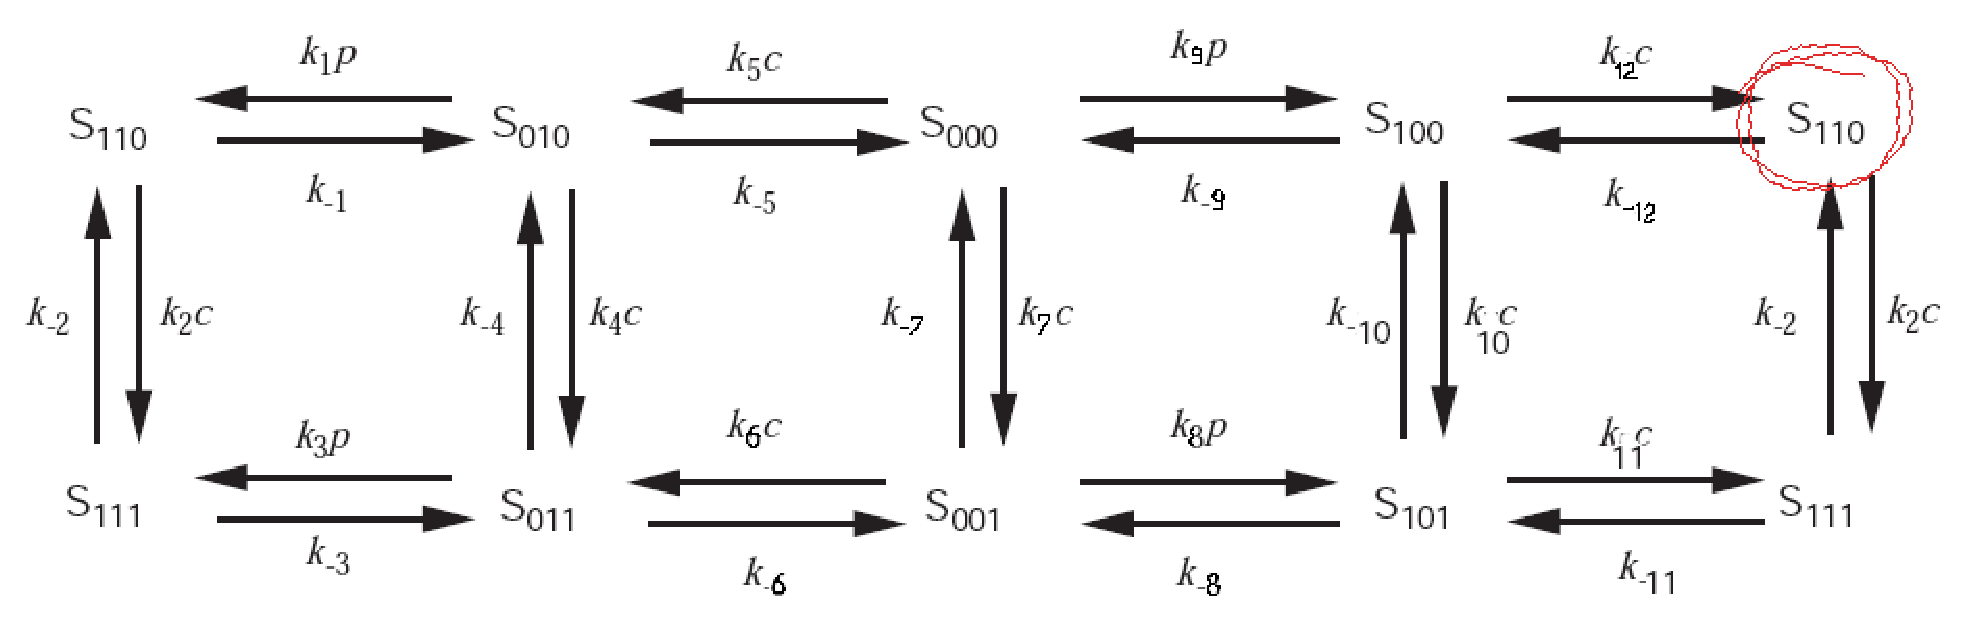
\includegraphics[height=4cm]{./images/IP3R_subunit_state.eps}}
 \centerline{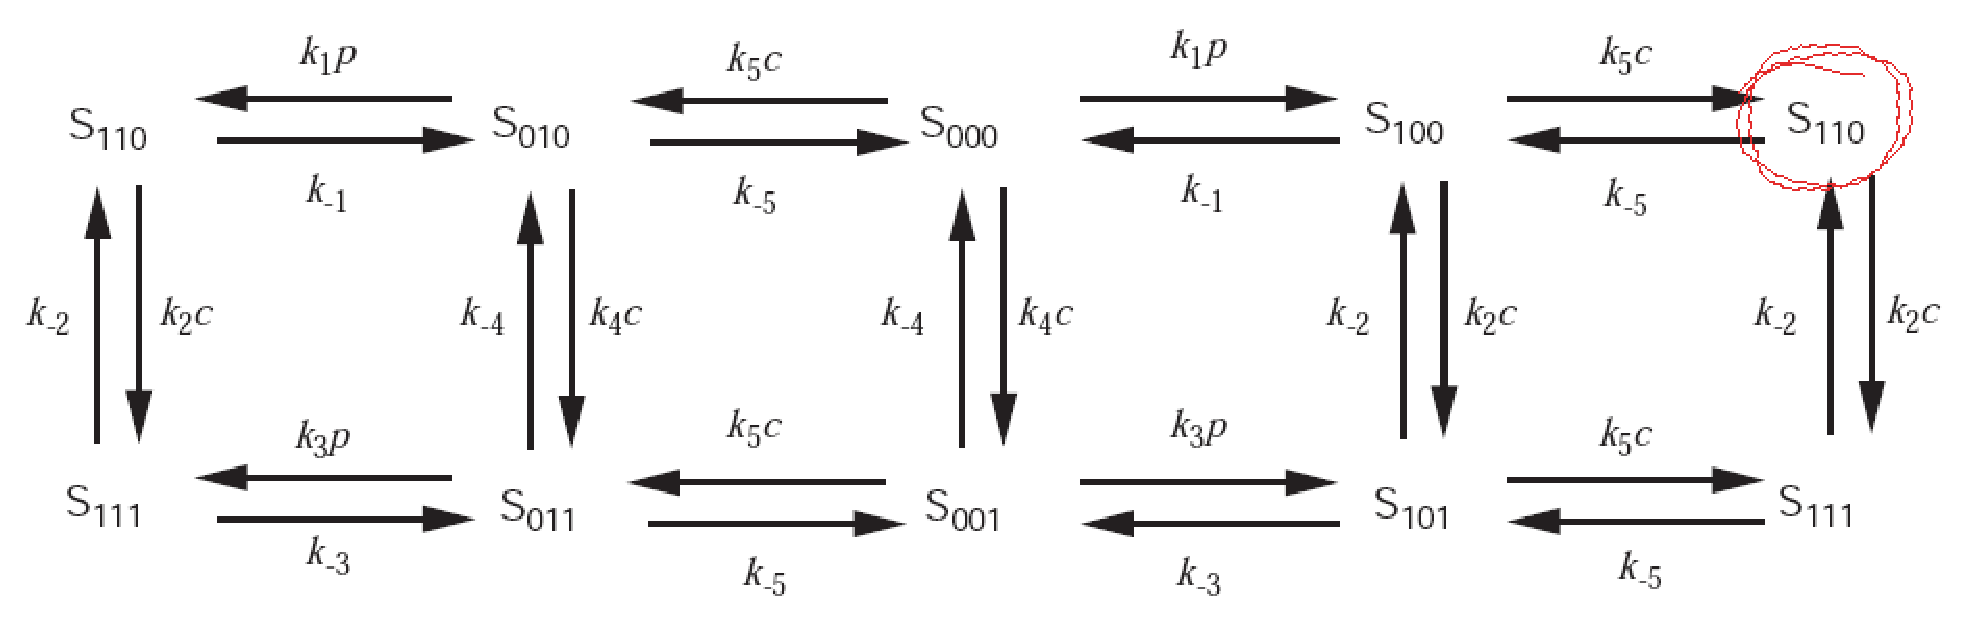
\includegraphics[height=4cm]{./images/DeYoung-Keizer_subunit.eps}}
 
 \caption{State transition diagram of a single IP3R subunit.  $c$
   denotes [\ce{Ca^2+}], $p$ denotes [IP3]. (A) complete form; (B) reduced form
   }
\label{fig:DYK_subunit_general}
\end{figure}

\subsection{Parameters}

In general, there will be 24 rate constants, as shown in
Fig.~\ref{fig:DYK_subunit_general}(A). De Young and Keizer simplify the model by
assuming that rate constants for IP3 binding are independent of whether or not
$\Ca$ is bound, and rate constants for $\Ca$ binding are independent of whether
or not IP3 are bound. Finally, the number of rate constants reduced from 24 to
10, as shown in Fig.~\ref{fig:DYK_subunit_general}(B).

% \begin{figure}[hbt]
%  \centerline{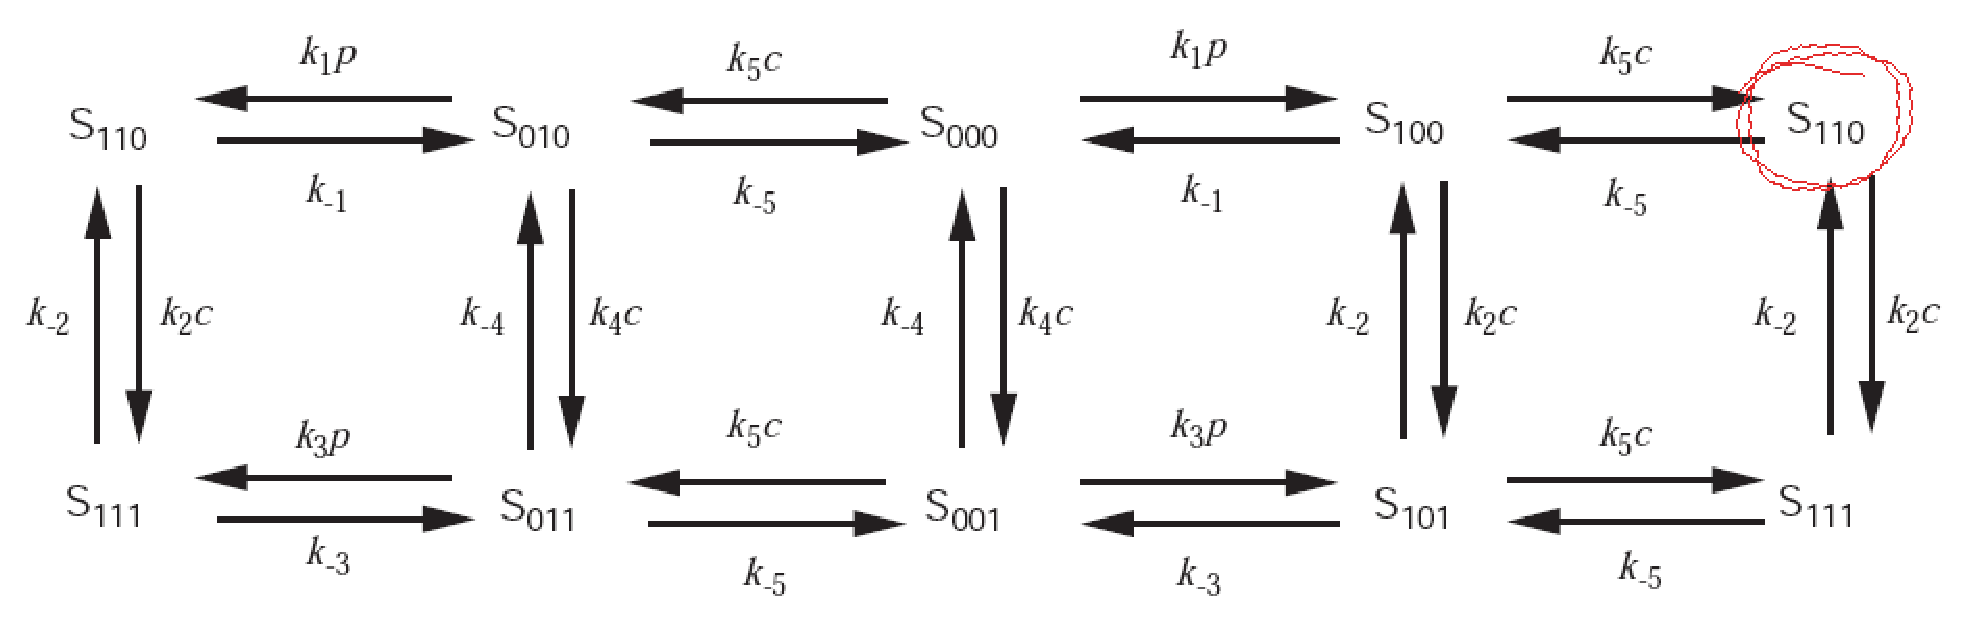
\includegraphics[height=4cm]{./images/DeYoung-Keizer_subunit.eps}}
% \caption{State transition diagram of a single subunit in De
%   Young-Keizer model. $c$ denotes [\ce{Ca^2+}], $p$ denotes [IP3].}
% \label{fig:DYK_subunit}
% \end{figure}
With 8 states, only 7 are independent and the other one can induced
from these 7 states based on the conservation of probability,
$\sum_{i,j,k}x_{ijk} = 1$. The 7 differential equations for these
fractions are based on {\it mass action kinetics}, as given below
% \begin{equation}
%   \label{eq:292}
%   \begin{split}
%     \frac{dx_{000}}{dt} &= k_{-5}x_{010} + k_{-1}x_{100} +
%     k_{-4}x_{001} - (k_5c+k_1p+k_4c)x_{000} \\
%     ... \\
%     \frac{dx_{110}}{dt} &= k_5cx_{100} + k_{-2}x_{111} + k_1px_{010} -(k_{-5}+k_2c+k_{-1})x_{110} \\
%   \end{split}
% \end{equation}
\begin{equation}
  \label{eq:292}
  \begin{split}
    \frac{dx_{000}}{dt} &= b_{5}x_{010} + b_{1}x_{100} +
    b_{4}x_{001} - (a_5c+a_1p+a_4c)x_{000} \\
    \frac{dx_{100}}{dt} &= b_{5}x_{110} + a_{1}px_{000} +
    b_{2}x_{101} - (b_1+a_2c+a_5c)x_{100} \\
    \frac{dx_{101}}{dt} &= b_{5}x_{111} + a_{2}cx_{100} +
    a_{3}px_{001} - (b_2+b_3+a_5c)x_{000} \\
    \frac{dx_{011}}{dt} &= a_{5}cx_{001} + a_4cx_{010} +
    b_{3}x_{111} - (b_5+b_4+a_3p)x_{000} \\
    \frac{dx_{010}}{dt} &= a_{5}cx_{000} + b_{1}x_{110} +
    b_{4}x_{011} - (a_5c+a_1p+a_4c)x_{000} \\
    \frac{dx_{001}}{dt} &= b_{5}x_{010} + a_{4}cx_{000} +
    b_{3}x_{101} - (a_5c+b_4+a_3p)x_{000} \\
     \frac{dx_{110}}{dt} &= a_5cx_{100} + b_{2}x_{111} + a_1px_{010} -(b_{5}+a_2c+b_{1})x_{110} \\
  \end{split}
\end{equation}
with $x_{ijk}$ is the fraction of subunits in the state $S_{ijk}$.
\textcolor{red}{In order to solve this model, we need to know $c,p$,
  and 10 other parameters $b_i,a_i$ ($i=1..5$)}. These 10 parameters
require 10 equations.

The schematic diagram in Fig. \ref{fig:DYK_subunit_general} (A) or (B) can be
represented in a cubic form given in Fig.~\ref{fig:DeYoung-Keizer_diagram} with
$a_i$'s are second-order rate constants
(Sect.\ref{sec:second-order-rate-constant}), $b_i$'s are first-order rate
constants. The model assume fast binding of activating $\Ca$ and slow binding of
inactivating  $\Ca$. Thus, the model incorporated in the magnitude of the rate
constants ($k_5>k_2, k_5>k_4$) or (for figure below) ($a_5>a_2$ and $a_5>a_4$).

\begin{figure}[hbt]
 \centerline{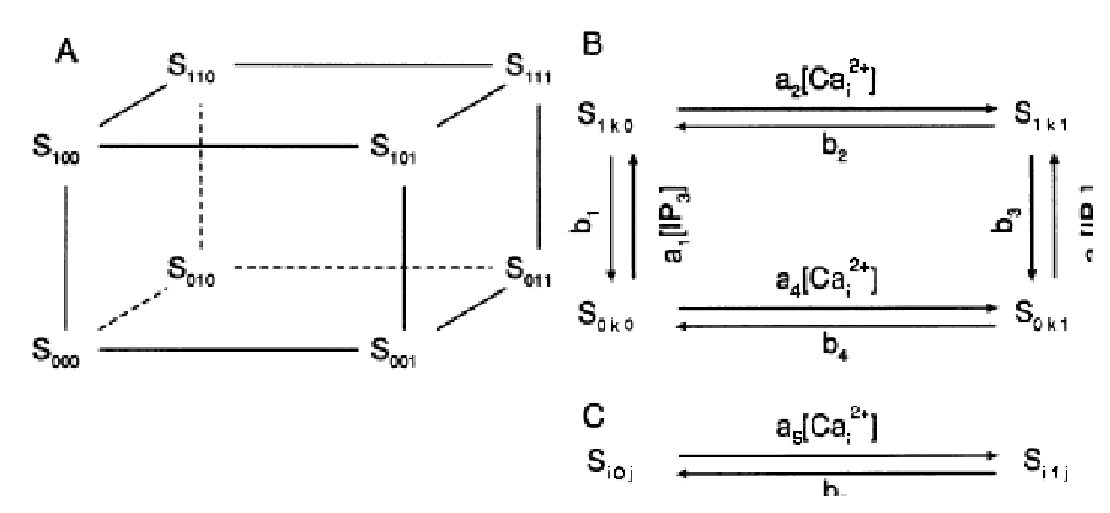
\includegraphics[height=4cm]{./images/DeYoung-Keizer_diagram.eps}}
\caption{De Young-Keizer schematic cubic diagram for a single subunit: (A) 8
possible states, (B) the kinetics of the front ($k=0$) and back ($k=1$) faces
of the cube in (A); (C) the kinetics for the transition between the front
and the back faces of the cube in (A)}
\label{fig:DeYoung-Keizer_diagram}
\end{figure}


% In order to determine these 12 parameters, we need to estimate them or with
% additional 12 equations. As $c$ and $p$ can be fixed, we only need 10
% equations.
De Young and Keizer used the experimental data from difference sources, and
obtained the following relations.
% As the [IP3] is fixed, it's the [\ce{Ca^2+}] that oscillates.
\begin{itemize}
\item At two different conditions: (1) no $\Ca$ and (2) $1\mu M$
  $\Ca$ by~\cite{joseph1989ip3}, the
  effective dissociation constant $K_d$ for IP3 binding to ER is
  $K_{D_1} = 145nM$, and $K_{D_2}=542nM$, respectively. By fixing
  $p=[IP3]=15nM$ (i.e. as the basal level), the equilibrium state
  $\frac{dx_{ijk}}{dt}=0$, has been fitted to the data to obtain the
  relationship.

\begin{equation}
  \label{eq:343}
  \begin{split}
    d_1 &= K_{D_1} - [IP3]\\
    d_3 &= (K_{D_2} - [IP3])(1+d_2) - d_1d_2
  \end{split}
\end{equation}
where $d_i = \frac{b_i}{a_i}$ and $[IP3] = 15 nM$. \textcolor{blue}{We
  now have 2 out of 10}.

% The dissociation constant $K_{D_i}$ for IP3 binding ($i=1$ or $3$) is
% $K_{D_i}=\frac{b_i}{a_i[IP3]}$. Fit to the experimental data, with De
% Young and Keizer obtained the

\end{itemize}


Based on the {\bf principle of microscopic reversibility}
(Sect.\ref{sec:microscopic-reversibility}),  consider this cyclic reaction as
shown in Fig.~\ref{fig:cyclic_reaction}, we always have this relation
\begin{equation}
  \label{eq:346}
  b_1\times a_4[\ce{Ca^2+}] \times a_3[IP3]\times b_2 =
  a_2[\ce{Ca^2+}]\times b_3 \times b_4 \times a_1 [IP3]
\end{equation}
or equivalently,
\begin{equation}
  \label{eq:347}
  \frac{b_2}{a_2}\frac{b_1}{a_2} = \frac{b_3}{a_3}\frac{b_4}{a_4}
\end{equation}

\begin{figure}[hbt]
 \centerline{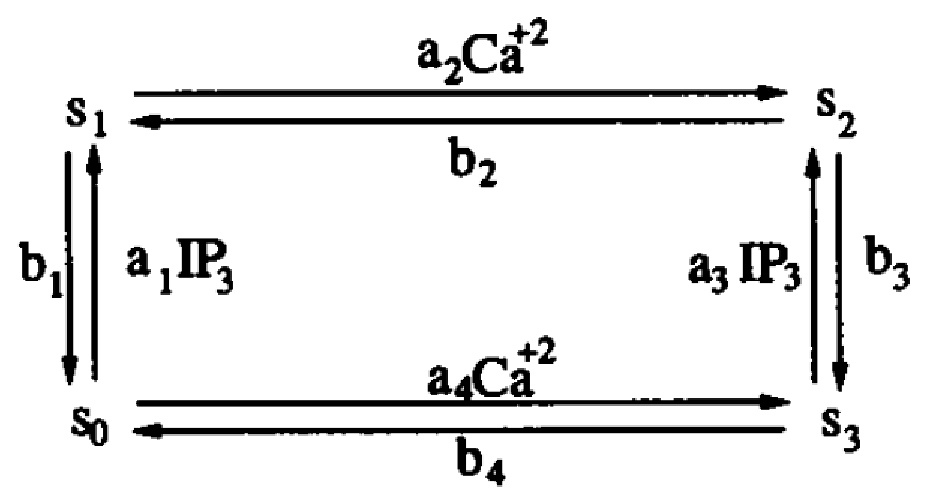
\includegraphics[height=3cm]{./images/cyclic_reaction.eps}}
\caption{An isolated cyclic reaction}
\label{fig:cyclic_reaction}
\end{figure}


% In order to estimate $a_i,b_i$, the author simply the model by
% assuming that $\Ca$ directly affects the binding of IP3. Thus, 
% each subunit is endowed 

Defining $d_i=b_i/a_i$, the dissociation constant $K_d$ with and
without $1\mu$M $\Ca$ is $K_{d1}=145nM$ and $K_{d2}=$542nM,
respectively. Accordingly, the relations were obtained
\begin{equation}
  \label{eq:345}
  \begin{split}
    d_1 &= K_{d1}-\overline{p} \\
    d_3 &= (K_{d2} - \overline{p})(1+d_2) - d_1d_2
  \end{split}
\end{equation}
with $\overline{p}=15nM$ is the concentration of labeled IP3. 



To close the model, we need one more differential equation for \ce{Ca^2+}
dynamics.  This will be discussed shortly.
 
\subsection{$[\Ca]_i$  oscillation}
\label{sec:ceca2-oscillation}

Sect.\ref{sec:calcium-oscill-waves} discusses calcium oscillations.
As shown in Fig.~\ref{fig:DYK_Ca2+}, the change
in calcium due to the efflux of $\Ca$ through IP3R, through leak
and the influx of $\Ca$ through ATP-dependent \ce{Ca^2+}
pumps. 
\begin{figure}[hbt]
 \centerline{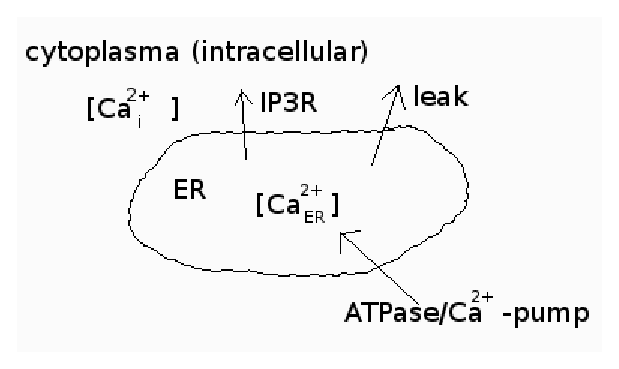
\includegraphics[height=5cm]{./images/DYK_Ca2+_dynamic.eps}}
\caption{The dynamics of $\Ca$  based on DeYoung-Keizer model. $c$
  is $[\ce{Ca_i^2+}]$, $c_{er}$ is $[\ce{Ca_{ER}^2+}]$.}
\label{fig:DYK_Ca2+}
\end{figure}

Based on the above analysis, dynamics of $c=[\Ca]_i$ is given
\begin{equation}
  \label{eq:344}
  \frac{dc}{dt} = \underbrace{r\times v_1(x_{110})^3(c_{er}-c)}_{\text{IP3R}}
  + \underbrace{r\times v_2(c_{er}-c)}_{\text{leak}} - 
 \underbrace{v_3\frac{c^2}{c^2+k_4^2}}_{\text{SERCA}}
\end{equation}
with $r$ is the volume ratio between that of the ER and that of the
cytosol, i.e. $\frac{V_{ER}}{V_{cyt}}$. Based on typical cell
parameters, $r$ was measured as $0.185$.

The maximum rate through each IP3R channel is $v_1$, through
leak is $v_2$, through pumps is $v_3$. Further, the amount of calcium
transport through IP3Rs is proportional to the number of open channels
and the difference in calcium concentration in cytoplasm and ER; the
efflux through the leak is proportional to the difference in calcium
concentration in cytoplasm and ER; finally, the influx through the
pumps is dependent on calcium cooperative binding of pumps with Hill
coefficients as 2, i.e.  it is proportional to $\frac{c^2}{c^2+k_p^2}$
with $k_p$ is dissociation constant of $\Ca$ binding to
pumps~\cite{carafoli1987cal}


\subsection{Complexity: Quasi-steady state approximation}
\label{sec:quasi-steady-state-IP3R}


NOTE: A fully general model of a single IP3R channel with 3 subunits would have
$8^3=512$ states, and only one open state: $110110110$.

{\bf Reduced the model}: 



\section{Li - Rinzel (1994)}
\label{sec:IP3R-Li-Rinzel-1994}

\citep{li1994} proposed a reduced 2-state model of the 9-state De Young-Keizer
model (Sect.\ref{sec:de-young-keizer}).

The method of multiple scales is used to solve the equations in a successive of
faster time scales to reduce the model to 2-state.
Assumptions
\begin{enumerate}
  \item IP3R is a tetramer; with 4 subunits

IP3R is open only when 3 out of 4 subunits are open.

  
  \item each subunit has 3 binding sites: IP3, Ca2+ activation, and Ca2+
  inactivation sites

  \item 3 time scales are separated: from fastest to slowest
  \begin{enumerate}
    \item IP3 regulation
    \item Ca2+ activation
    \item Ca2+ inactivation
  \end{enumerate}
  
  \item \textcolor{red}{different gating processes are independent from each
  other}, i.e.
  the rate of Ca2+ binding at one gating site is independent from the occupancy
  at the other two binding sites
\end{enumerate}



% There are 3 different time-scales
% \begin{enumerate}
%   \item IP3 regulation
%   \item Ca2+ activation
%   \item Ca2+ inactivation
% \end{enumerate}

\begin{equation}
J_\text{IP3R} = \frac{V_\er}{V_\cyto} \times v_{ip3r} \times m_\infty^3
\times n_\infty^3 \times h^3 \times ([\Ca]_\er - [\Ca]_i)
\end{equation}
with $c_1 = V_\er/V_\cyto$ is volume ratio of compartments (e.g. 
$c_1=0.185$); $v_{ip3r}=6^10^{-3}$ is transfer rate (1/msec), i.e. 6s$^{-1}$.
 
The first two gating variables $m_\infty, n_\infty$ represents the fast-binding
(instantaneous) of IP3 and Ca2+-activation, respectively.
\begin{equation}
m_\infty = \left\{ \frac{[IP3]}{[IP3] + d_1} \right\} \qquad; n_\infty = \left\{
\frac{[\Ca]}{[\Ca] + d_5} \right\}
% \begin{split}
% m_\infty = \left\{ \frac{[IP3]}{[IP3] + d_1} \right\} \\
% n_\infty = \left\{ \frac{[\Ca]}{[\Ca] + d_5} \right\}
% \end{split}
\end{equation}
with $d_1=0.13\muM$; $d_5=0.08234\muM$

The slow inactivation
variable $h$ represents Ca2+-dependent inactivation process
\begin{equation}
\begin{split}
\frac{dh}{dt} = \frac{h_\infty - h}{\tau_h} = \alpha_h \times (1-h) - \beta_h
\times h
\end{split}
\end{equation}
which depends on both the concentration of IP3 and and Ca2+ in the rate
constants
\begin{equation}
\begin{split}
\alpha_h = a_2 d_2 \frac{[IP3] + d_1}{[IP3] + d_3} \\
\beta_h = a_2 [\Ca] \\
\tau_h = \frac{1}{a_2 (Q_2 + [\Ca]_i)} \\
h_\infty = \frac{Q_2}{Q_2 + [\Ca]_i} \\
Q_2 = d_2 \frac{[IP3] + d_1}{[IP3] + d_3}
\end{split}
\end{equation}
with $d_1=0.13\muM; d_2=1.049\muM$; $d_3=0.9434\muM$%; $d_5=0.08234\muM$; 
and $a_2 = 0.2\times 10^{-3}$ (1/($\muM$.ms)).

\begin{equation}
\frac{d[\Ca]_i}{dt}  = J_\text{IP3R} - I_\text{pump} + I_\text{ER,leak}
\end{equation}
with 
\def\pump{{\text{pump}}}
\begin{equation}
\begin{split}
I_\text{pump} = v_\text{pump} \times \frac{([\Ca]_i)^2}{([\Ca]_i)^2 + K_\pump^2}
\\
I_\text{ER,leak} = c_1 \times v_{\text{ER,leak}} \times ([\Ca]_\er - [\Ca]_i)
\end{split}
\end{equation}
with $v_\text{ER,leak}=0.11\times 10^{-3}$ (1/ms); 
$v_\pump=0.9\times 10^{-3}$
($\muM$/ms); $K_\pump = 0.1 \muM$


\subsection{model}

The stochastic Li-Rinzel model for a cluster larger than 10 channels reproduces
the data using in De Young-Keizer (Sect.\ref{sec:de-young-keizer}) pretty well.

NOTE: $h=1$ means channel open (which represent the non-inactivating member);
and $h=0$ means closed IP3R.

The three non-inactivation gate $h$ can be assumed to be in either 0 or 1 state.
The switching can be approximated using a 2-state Markov process with opening
rate $\alpha_h$ and closing rate $\beta_h$.

In a cluster of $N$ channel, 
\begin{equation}
I_\text{IP3R} = c_1 v_\text{IP3R} m_\infty^3 n_\infty^3
\frac{N_\open}{N}([\Ca]_\er - [\Ca]_i)
\end{equation}
A channel is open if number of $h$-gate is 3 or more.

\section{Swillens-\ldots-Dupont (1998) - stochastic simulation single IP3R}
\label{sec:Swillens_1998_singleIP3R}

\citep{swillen1998sss} showed that IP3R is capable of repetitive opening, i.e.
burst of activity and the result was reminiscent of the relatively long-duration
experimental calcium blips (Sect.\ref{sec:blips}).

\begin{figure}[hbt]
 \centerline{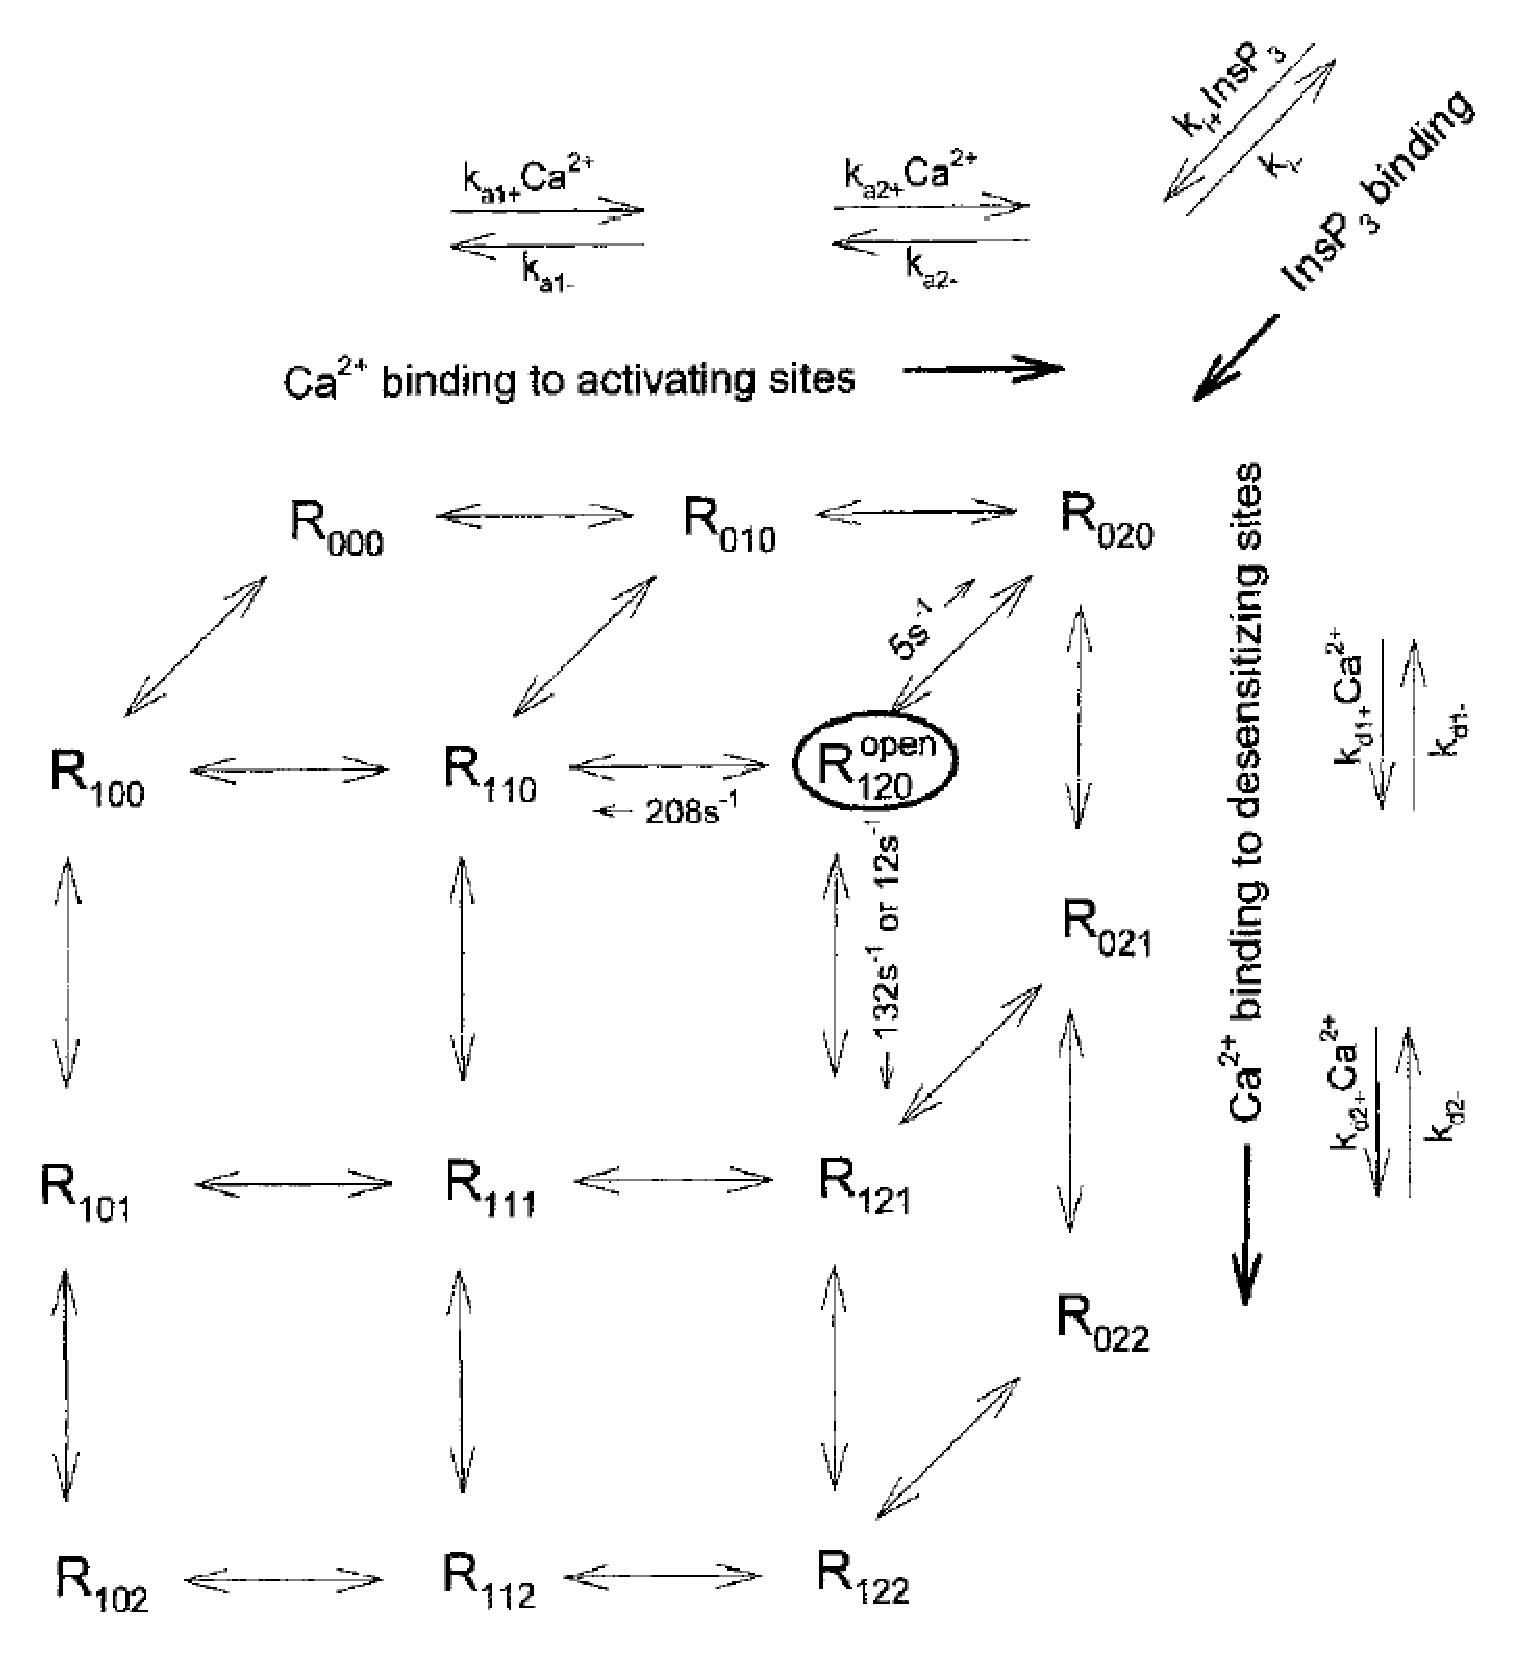
\includegraphics[height=3.5cm]{./images/IP3R-Swillens-Dupont-1998.eps}}
\caption{Model with single IP3R channel}
\label{fig:IP3R-Swillens-Dupont-1998}
\end{figure}


They proposed a single channel model, Fig.\ref{fig:IP3R-Swillens-Dupont-1998},
with
\begin{enumerate}
  \item single IP3 binding site

It is assumed IP3 binding is not-cooperative; and IP3 binding is not dependent
upon $\Ca$ binding.
  
  \item 2 calcium ion activation binding sites
  
  \item 2 calcium ion inactivation binding sites
  
  \item there is cooperative in calcium binding to activation site; and
  inactivate site; but it is assumed that there is no allosteric interaciton
  between these different sites (Sect.\ref{sec:allosteric-coupling})

  \item NOTE: $R_{ijk}$ refers to a state of the IP3R with $i$ can be 0 or 1;
  $j$ can be 0,1, or 2; and $k$ can be 0, 1 or 2.


  \item the only open state is $R_{120}$:
  
NOTE: the channel IP3R is in open state only when IP3 is bound ($i=1$); and
calcium ions present at both activation site ($j=2$) and there is no calcium
bound at any inactivation site ($k=0$).
  
  \item calcium-level is considered at the mouth, which can be much higher
  than the bulk cytosolic calcium.
\end{enumerate}

In their model, single channel maximum opening probability is 
\begin{itemize}
  \item 0.05 with single channel current 1.1 pA
  
  \item 0.2 with single channel current 0.1 pA
\end{itemize} 


\section{** Sneyd-Dufour (2002): IP3R type 2}
\label{sec:sneyd-dufour_IP3R_2002}


The model developed by Sneyd and Dufour is for IP3R type 2
\citep{sneyd2002ip3r2}..

IMPORTANT:
\begin{enumerate}
  \item  removed the assumption of independent binding of calcium and IP3

The binding is sequential, and IP3 has to bind first.
  
  \item three inactivated states: I1, I2 and S.

States I1 and I2 have calcium bound to the same inactivating site.  
State I2 also has IP3 binding. So, state I1 is necessary for the channel to
switch to inactivated state, in the absence of IP3.

State I2 is necessary so that the channel can switch to inactivated state by
calcium.

State S is necessary so that an open channel can inactivate in the absence of
calcium (to binding to inactivating site).

  \item  
\end{enumerate}


\section{Smith et al. (2002): microdomain Calcium}

Most model of IP3 assumed a well-mixed of calcium in the bulk which ignore
calcium concentration gradient, diffusion. This is not valid for very large cell
like cardiac myocyte and Xenopus oocytes which exhibit dramatic calcium wave
(Sect.\ref{sec:calcium-oscill-waves}).

Also, in small region, notably the microdomain in the ER-PM junction
(Sect.\ref{sec:junction-ER-plasmamembrane}) where calcium elevation can be a few
order of magnitudes than those in bulk cytosol. 

Smith (2002) re-fitted the De Young - Keizer model using domain calcium
concentration. 

%https://books.google.com/books?id=Cy67CwAAQBAJ&pg=PA134&lpg=PA134&dq=Li+Rinzel+IP3R&source=bl&ots=CI7xzqbAgN&sig=SqGeQjnKzHnCQ5sVxw5laoRwq7c&hl=en&sa=X&ved=0ahUKEwiW0Jeby-LPAhXCZCYKHcJBBeMQ6AEISjAI#v=onepage&q=Li%20Rinzel%20IP3R&f=false

%https://books.google.com/books?id=bXrMBQAAQBAJ&pg=PA369&lpg=PA369&dq=Smith+2002+IP3R&source=bl&ots=oluyJ2NdlS&sig=_nHba6Cjyrfo7Arqq3_-Vw0O-Rk&hl=en&sa=X&ved=0ahUKEwj6ooHi0uLPAhVB4iYKHRBHD1kQ6AEIHDAA#v=onepage&q=Smith%202002%20IP3R&f=false


\section{** Mak-McBride-Foskett (2003) - allosteric modelling: IP3R type 1}
\label{sec:Mak_2003_IP3R}

Mak's group conducted several studies of the native IP3R channel from insect Sf9
cells, which has a primary sequence most closely related to the type 1 IP3R
isoform in vertebrate cells. They confirmed that the inhibition of IP3R at high
calcium level is calmodulin-independent. 
Also, they suggest that there are two calcium inactivation binding sites; and
only one of that is IP3 sensitive.


\citep{mak2003} developed a Markov-based model that can replicate not only Ca2+
dependency of Po, but also IP3 dependency of Po. 

The model requires 14 parameters

\section{Fraiman-Dawson (2004) - luminal calcium binding site}
\label{sec:Fraiman_2004_IP3R}

\citep{fraiman2004mip3} 

\section{Sneyd-Dufour (2005)}

\citep{sneyd2005ip3r}


\section{Shuai-\ldots-Paker (2007)}
\label{sec:shuai_2007}

\citep{shuai2007kmip3r} model is derived based on De Young-Keizer model
(Sect.\ref{sec:de-young-keizer}). 

\section{Shuai-Pearson-Parker (2008) - $\Ca$ feedback on channel}
\label{sec:shuai_2008_Ca-feedback}

Steady-state gating properties of IP3R have been extensively studies and modeled
under the assumption of fixed $[\mIPthree]$ and fixed $[\Ca]$.
\textcolor{red}{The question is how $\Ca$ through the channel provide a feedback
on activating and inhibiting the $\Ca$-binding sites}. \citep{shuai2008} carried
the study on monomeric and tetrameric \tIPthreeR models. Suggested results:

\begin{enumerate}
  
  \item activation effect: stationary cytosolic $\Ca$ buffers play a major role
  in keeping $\Ca$ so that it slow the decreasing of local $\Ca$ in microdomain
  after closure, allowing self-activation of the channels, promoting {\bf
  burst}-like reopenings by the rebinding of $\Ca$ to the activating site

  \item inhibitory effect: independent of stationary buffers, but strongly
  dependent upon the location of inhibitory $\Ca$ binding site in relation to
  channel pore. 
\end{enumerate}

\section{Ullah-Mak-Pearson (2012): IPR3 type I}
\label{sec:IP3R1-Ullah2012}
\label{sec:Ullah-Mak-Pearson-2012-IP3R}

\citep{ullah2012} developed a Markov-based model for IP3R type 1 using data
from insect Sf9 cells.
\begin{itemize}
  \item 3 open states
  \item 9 closed states
\end{itemize}
with 28 parameters.

Instead of looking at the channel as individual subunits, which make requires
making assumptions about sequential or random binding, Ullah et al.
looks at IP3R as an oligomer with 4 IP3-binding sites.

{\bf Cooperative model} (CM): the authors construct a CM model with
cooperativity in the IP3-binding dynamic.

DYKM (DeYoung-Keizer Model - Sect.\ref{sec:de-young-keizer}) yields a somewhat
higher likelihood for the Po data than the CM.
The DYKM does a very good job reproducing the Po data from Sf9 cells. However,
it does not compete well with the CM when the recent kinetic data are taken into
account




\section{Siekmann-\ldots-Sneyd (2012)}

\citep{siekmann2012} developed Markov model for types I and II IP3R using
single-channel data set. The kinetics of the model depend on the concentrations
of [IP3], [ATP], and [$\Ca$]. The models are mode-switching, each mode is
ligand-independent, and the transitions between modes are ligand-dependent. 

%%% Local Variables: 
%%% mode: latex
%%% TeX-master: "mainfile"
%%% End: 
